\documentclass[letterpaper,openany,twoside,twocolumn]{book}

\newcommand{\PATH}{../../../../../}

\usepackage[justified]{\PATH dndtemplate/dnd}
\usepackage{\PATH monsters/stylesheets/monster_stylesheet}
\usepackage{\PATH monsters/stylesheets/shadowfy}

\usepackage[english]{babel}
\usepackage[utf8]{inputenc}

%\newcommand{\entryfont}{\DndFontStatBlockBody} & uses the default font provided by the LaTeX DnD-Template
\newfontfamily\entryfont{Kalam}[Path=\PATH template/fonts/,Extension=.ttf,UprightFont=Kalam-Regular,BoldFont=Kalam-Bold] % requires XeLaTeX or LuaTeX

\begin{document}
	\graphicspath{{./images},{./monsters/Toxicore_Basilisk/images}}

\MonsterSheetGeometry

% --------------------------------------------------------------------------------------------------- %
% ################################################################################################### %
% #-#-#-#-#-#-#-#-#-#-#-#-#-#-# Monster-Sheet with two Smaller Pictures #-#-#-#-#-#-#-#-#-#-#-#-#-#-# %
% ################################################################################################### %
% --------------------------------------------------------------------------------------------------- %

\chapter*{Toxicore Basilisk}
\stepcounter{chapter}
\addcontentsline{toc}{chapter}{\protect\numberline{\thechapter}Toxicore Basilisk}

\begin{tikzpicture}[overlay, remember picture, inner sep=0pt, outer sep=0pt, path fading=fade down]%
	\node (posSW) at (current page text area.south west) {};%
	\node[below left=30pt and 1.25cm of posSW, anchor=south west] (cornerSW) {%
		\begin{minipage}{\paperwidth}%%
        	\centering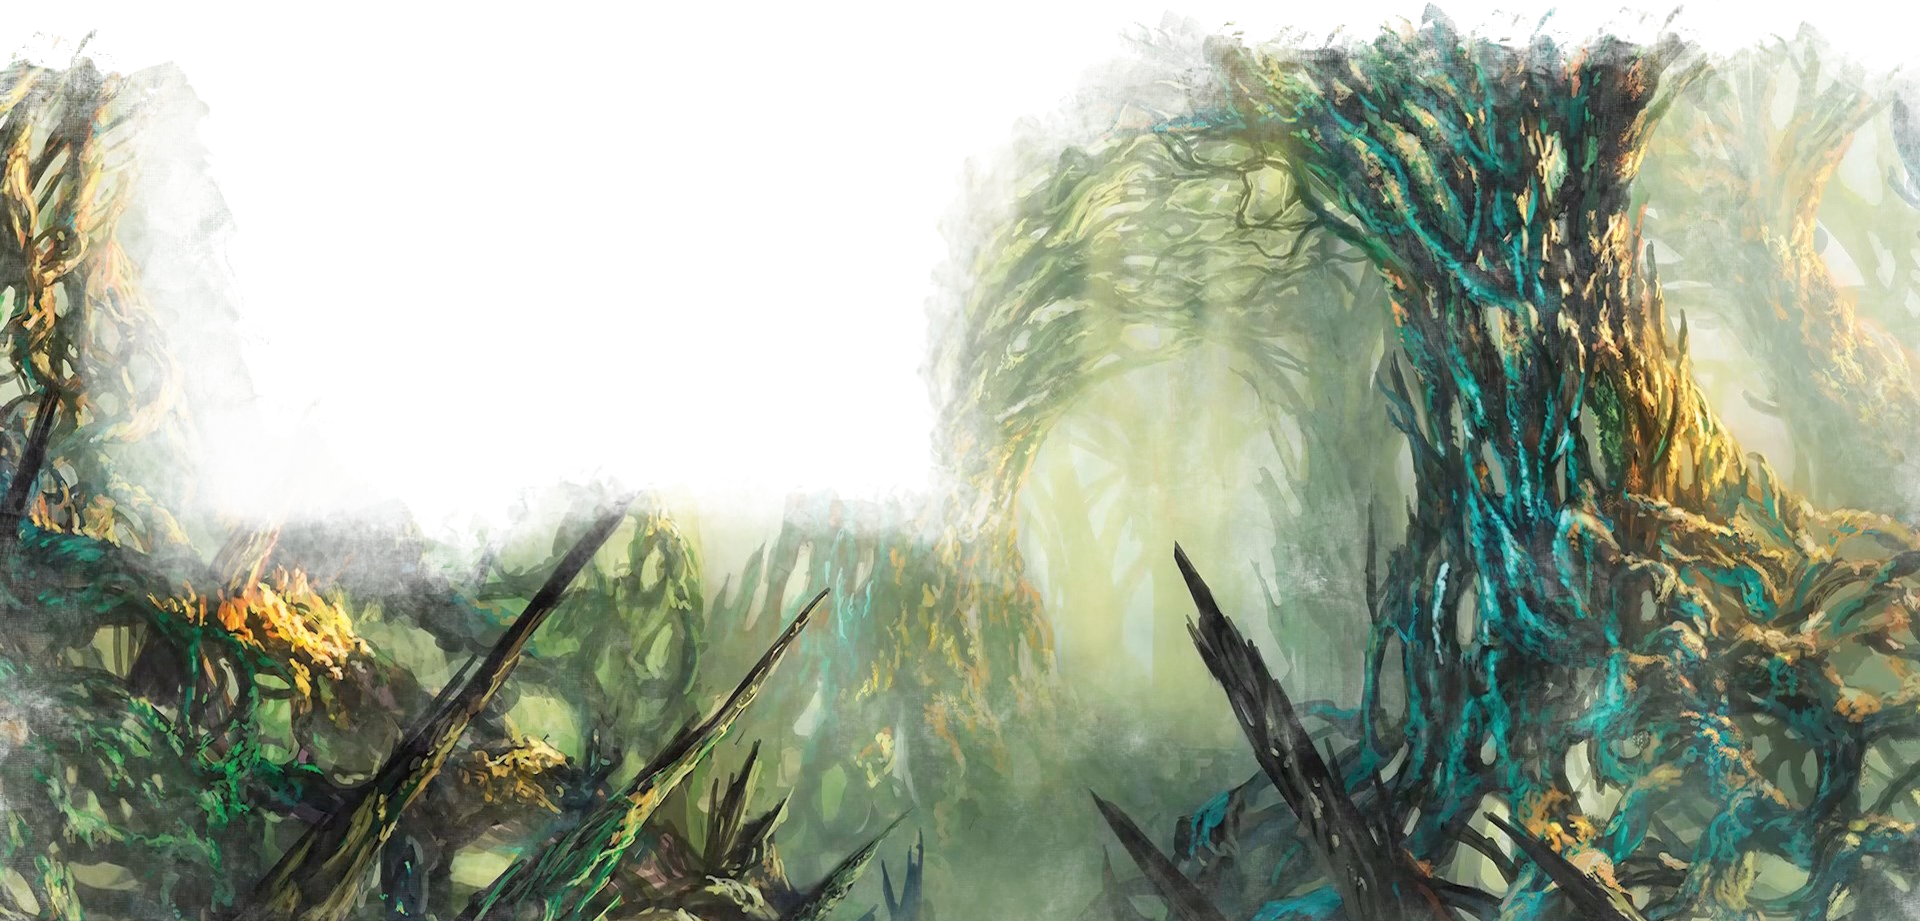
\includegraphics[width=\paperwidth, height=300pt]{Toxic_Forest.png}%
      	\end{minipage}%
	};%
\end{tikzpicture}%
\addImageDBEntry{ToxicoreBasilisk1}{Page \thepage}{Background Art}{https://www.artofmtg.com/art/the-hunters-maze/}{The Hunter’s Maze MtG Art from Phyrexia: All Will Be One}{Alayna Danner}%

\vspace*{-2.4\fontdimen6\font}

\entryfont \noindent \DndDropCapLine{A} fearsome reptilian abomination, the Toxicore Basilisk possesses a bionic appearance with scales resembling polished steel. These metallic plates reflect light in a mesmerizing display, giving the creature an otherworldly, almost mechanical aura. Its massive form, accentuated by a vivid green hue that seems to pulsate with an eerie glow, instills both awe and dread in those who behold it.
\paragraph{Toxic Emanation} Known throughout the land for its toxic nature, the Toxicore Basilisk has the unique ability to generate a highly potent black ichor. This toxic substance not only eats away at the very fabric of the environment, leaving a trail of decay and corruption, but also possesses hazardous properties that pose a grave threat to any living beings it touches. The mere proximity to this creature can leave a lasting impact, its very presence tainting the air with darkness.

\paragraph{Lethal Variations} Within the Toxicore Basilisk species, two distinct adult variations exist, each with its own terrifying attributes. The first variation, often referred to as the Bladed Basilisk, resembles a nightmarish fusion of a Tyrannosaurus and an insect. Jagged and imposing blades extend from its body and head, serving as deadly weapons that strike fear into the hearts of its adversaries. With a lightning-fast charge, the Bladed Basilisk unleashes a barrage of devastating attacks, utilizing its razor-sharp blades to slice through even the toughest defenses.

In stark contrast, the second variant, known as the Insectoid Basilisk, takes on the form of a massive insect with an elongated body. Its steel-like exoskeleton glistens with an uncanny sheen, while scythe-like appendages extend from its head and limbs. Agile and nimble, the Insectoid Basilisk swiftly maneuvers across the battlefield, delivering precise and lethal strikes with its deadly scythes. It leaves behind a trail of devastation, deep wounds marking its path.

Even in its infant stage, the Toxicore Basilisk commands attention. Known as the Toxicore Hatchling Salamanderids, these young creatures bear the resemblance of salamanders, yet possess insect-like mandibles on their heads. Though not as developed as their adult counterparts, these hatchlings display remarkable tenacity and a penchant for delivering painful bites. They possess an instinctual ability to defend themselves, ensuring their survival from an early age.

\paragraph{Unyielding Dread} Protected by its formidable steel-like scales, the Toxicore Basilisk presents an imposing challenge for any who dare to face it. Its toxic abilities, coupled with its lethal prowess and bionic appearance, make it a force to be reckoned with. Legends and cautionary tales abound, warning of the devastation left in the wake of this monstrous creature's path.

\vfill\eject % cammand to break to next column

% Monster stat block
\vspace*{2.6cm}\begin{DndMonster}[width=0.5\textwidth]{Toxicoreling}
    \DndMonsterType{Small Abomination, chaotic evil}

    % If you want to use commas in the key values, enclose the values in braces.
    \DndMonsterBasics[
        armor-class = {14 (natural armor)},
        hit-points  = {\DndDice{3d6 + 6}},
        speed       = {30 ft., climb 25 ft.},
    ]

    \DndMonsterAbilityScores[
        str = 10,
        dex = 16,
        con = 14,
        int = 6,
        wis = 12,
        cha = 6,
    ]

    \DndMonsterDetails[
        %saving-throws = {Str +0, Dex +0, Con +0, Int +0, Wis +0, Cha +0},
        skills = {Perception +3, Stealth +6},
        %damage-vulnerabilities = {cold},
        %damage-resistances = {bludgeoning, piercing, and slashing from nonmagical attacks},
        %damage-immunities = {cold},
        senses = {Darkvision 60ft., passive Perception 13},
        %condition-immunities = {frightened, poisoned},
        languages = {-},
        challenge = 1/2,
    ]
    
    \DndMonsterAction{Amphibious}
    The Toxicore Hatchling can breathe both air and water.
    
    \DndMonsterAction{Evasive Maneuvers}
    The Toxicore Hatchling can take the Dodge action as a bonus action on its turn.
    
    \DndMonsterAction{Nimble Escape}
    The Toxicore Hatchling can take the Disengage or Hide action as a bonus action on each of its turns.
	
	\DndMonsterSection{Actions}	
	\DndMonsterAttack[
      name=Toxic Bite,
      distance=melee, % valid options are in the set {both,melee,ranged},
      %type=weapon, %valid options are in the set {weapon,spell}
      mod=+5,
      reach=5,
      %range=20/60,
      targets=one target,
      dmg=\DndDice{1d6 + 3},
      dmg-type=piercing,
      plus-dmg=\DndDice{1d6},
      plus-dmg-type=poison,
      %or-dmg=,
      %or-dmg-when=,
      extra={. The target must succeed on a DC 12 Constitution saving throw or be poisoned for 1 minute. The poisoned creature can repeat the saving throw at the end of each of its turns, ending the effect on itself on a success},
    ]
    
    \DndMonsterAttack[
      name=Venomous Tail Whiplash,
      distance=melee, % valid options are in the set {both,melee,ranged},
      %type=weapon, %valid options are in the set {weapon,spell}
      mod=+5,
      reach=10,
      targets=one target,
      dmg=\DndDice{1d4 + 3},
      dmg-type=bludgeoning,
      plus-dmg=\DndDice{1d6},
      plus-dmg-type=poison,
      %or-dmg=,
      %or-dmg-when=,
      %extra=,
    ]
    
    \DndMonsterAttack[
      name=Toxic Spittle (Recharge 5-6),
      distance=ranged, % valid options are in the set {both,melee,ranged},
      %type=weapon, %valid options are in the set {weapon,spell}
      mod=+5,
      reach=20/60,
      targets=one target,
      dmg=\DndDice{1d4 + 3},
      dmg-type=acid,
      plus-dmg=\DndDice{1d6},
      plus-dmg-type=poison,
      %or-dmg=,
      %or-dmg-when=,
      %extra=,
    ]
      
\end{DndMonster}

\vspace*{-17cm}\hspace*{5.75cm}\begin{tikzpicture}[overlay, remember picture, inner sep=0pt, outer sep=0pt, path fading=fade down]%
		\node (picture) at (0,0) {\includegraphics[width=1.2\columnwidth, height=280pt, keepaspectratio]{Toxicoreling.png}};%
\end{tikzpicture}%
\addImageDBEntry{ToxicoreBasilisk2}{Page \thepage}{MonsterArt}{https://mtg.cardsrealm.com/en-us/card/ichorspit-basilisk}{Ichorspit Basilisk MtG Art from Phyrexia: All Will Be One}{Joe Slucher}%

\newpage

\hfill\\\vspace*{6cm}

% Monster stat block
\begin{DndMonster}[width=0.5\textwidth]{Scythera~~~~~~~Basilisk}
    \DndMonsterType{Large Abomination,~~~~~~~~~~~chaotic evil}

    % If you want to use commas in the key values, enclose the values in braces.
    \DndMonsterBasics[
        armor-class = {16 (natural armor)},
        hit-points  = {\DndDice{10d10 + 40}},
        speed       = {40 ft.},
    ]

    \DndMonsterAbilityScores[
        str = 18,
        dex = 14,
        con = 18,
        int = 4,
        wis = 12,
        cha = 6,
    ]

    \DndMonsterDetails[
        %saving-throws = {Str +0, Dex +0, Con +0, Int +0, Wis +0, Cha +0},
        skills = {Perception +5, Stealth +4},
        %damage-vulnerabilities = {fire},
        damage-resistances = {Bludgeoning, Piercing, and Slashing from Nonmagical Attacks},
        %damage-immunities = {exhaustion, frightened, poisoned},
        senses = {Darkvision 60ft, passive Perception 15},
        %condition-immunities = {frightened, poisoned},
        languages = {-},
        challenge = 6,
    ]
	
	\DndMonsterAction{Steelhide}
    The Scythera Basilisk has resistance to piercing, slashing, and bludgeoning damage from nonmagical attacks that aren't silvered.
    
    \DndMonsterAction{Keen Senses}
    The Scythera Basilisk has advantage on Wisdom (Perception) checks that rely on sight or smell.
    
    \DndMonsterAction{Toxic Ichor}
    A 10-foot radius around the Scythera Basilisk is filled with a toxic ichor. Any creature that starts its turn within this radius must make a DC 14 Constitution saving throw, taking \DndDice{3d6} poison damage on a failed save, or half as much damage on a successful one.
	
	\DndMonsterSection{Actions}
	
	\DndMonsterAction{Multiattack}
	The Scythera Basilisk makes two scythe attacks or one Scythe attack and one Poisonous Sting attack.
	
	\DndMonsterAttack[
      name=Scythe,
      distance=melee, % valid options are in the set {both,melee,ranged},
      %type=weapon, %valid options are in the set {weapon,spell}
      mod=+7,
      reach=10,
      %range=20/60,
      targets=one target,
      dmg=\DndDice{2d8 + 4},
      dmg-type=slashing,
      %plus-dmg=,
      %plus-dmg-type=,
      %or-dmg=,
      %or-dmg-when=,
      %extra=,
    ]
    
    \DndMonsterAttack[
      name=Poisonous Sting,
      distance=melee, % valid options are in the set {both,melee,ranged},
      %type=weapon, %valid options are in the set {weapon,spell}
      mod=+7,
      reach=5,
      %range=20/60,
      targets=one target,
      dmg=\DndDice{2d6 + 4},
      dmg-type=piercing,
      plus-dmg=\DndDice{2d6},
      plus-dmg-type=poison,
      %or-dmg=,
      %or-dmg-when=,
      extra={. The target must succeed on a DC 14 Constitution saving throw or be poisoned for 1 minute. The poisoned creature can repeat the saving throw at the end of each of its turns, ending the effect on itself on a success},
    ]
	
	\DndMonsterAction{Venomous Burst (Recharge 5-6)}
	The Scythera Basilisk releases a burst of toxic energy in a 15-foot cone. Each creature in that area must make a DC 14 Constitution saving throw, taking \DndDice{6d6} poison damage on a failed save, or half as much damage on a successful one.
      
\end{DndMonster}

\vfill\eject % cammand to break to next column

% Monster stat block
\begin{DndMonster}[width=0.5\textwidth +0.5em]{Bladescale Basilisk}
    \DndMonsterType{Huge Abomination, chaotic evil}

    % If you want to use commas in the key values, enclose the values in braces.
    \DndMonsterBasics[
        armor-class = {16 (natural armor)},
        hit-points  = {\DndDice{14d12 + 56}},
        speed       = {40 ft.},
    ]
    
    \renewcommand{\AbilityScoreSpacer}{~}

    \DndMonsterAbilityScores[
        str = 22,
        dex = 14,
        con = 18,
        int = 5,
        wis = 10,
        cha = 7,
    ]

    \DndMonsterDetails[
        %saving-throws = {Str +0, Dex +0, Con +0, Int +0, Wis +0, Cha +0},
        skills = {Perception +4},
        %damage-vulnerabilities = {fire},
        damage-resistances = {Bludgeoning, Piercing, and Slashing from Nonmagical Attacks},
        %damage-immunities = {exhaustion, frightened, poisoned},
        senses = {Darkvision 60ft, passive Perception 14},
        %condition-immunities = {frightened, poisoned},
        languages = {-},
        challenge = 9,
    ]
    
    \DndMonsterAction{Steelhide}
    The Scythera Basilisk has resistance to piercing, slashing, and bludgeoning damage from nonmagical attacks that aren't silvered.
    
    \DndMonsterAction{Keen Senses}
    The Scythera Basilisk has advantage on Wisdom (Perception) checks that rely on sight or smell.
    
    \DndMonsterAction{Blade Armor}
    Whenever a creature hits the Bladescale Basilisk with a melee attack while within 5 feet of it, the attacker takes \DndDice{2d6} slashing damage.
	
	\DndMonsterSection{Actions}
	
	\DndMonsterAction{Multiattack}
	The Bladescale Basilisk makes two claw attacks and one bite attack.
	
	\DndMonsterAttack[
      name=Claw,
      distance=melee, % valid options are in the set {both,melee,ranged},
      %type=weapon, %valid options are in the set {weapon,spell}
      mod=+9,
      reach=10,
      %range=20/60,
      targets=one target,
      dmg=\DndDice{2d6 + 7},
      dmg-type=slashing,
      %plus-dmg=,
      %plus-dmg-type=,
      %or-dmg=,
      %or-dmg-when=,
      %extra=,
    ]
    
    \DndMonsterAttack[
      name=Bite,
      distance=melee, % valid options are in the set {both,melee,ranged},
      %type=weapon, %valid options are in the set {weapon,spell}
      mod=+9,
      reach=5,
      %range=20/60,
      targets=one target,
      dmg=\DndDice{2d10 + 6},
      dmg-type=slashing,
      plus-dmg= \DndDice{3d6},
      plus-dmg-type=poison,
      %or-dmg=,
      %or-dmg-when=,
      extra={. The target must succeed on a DC 16 Constitution saving throw or be poisoned for 1 minute. The poisoned creature can repeat the saving throw at the end of each of its turns, ending the effect on itself on a success},
    ]
    
    \DndMonsterAction{Razor Gale (Recharge 5-6)}
	The Bladescale Basilisk whips its tail in a wide arc, sending forth a flurry of razor-sharp scales. Each creature within a 20-foot cone must make a DC 16 Dexterity saving throw, taking \DndDice{8d6} slashing damage on a failed save, or half as much damage on a successful one.

	\DndMonsterAction{Razor Bash (Recharge 5-6)}
	The Bladescale Basilisk charges forward in a straight line, bashing everything and everyone in its path. Each creature in a 60-foot line must make a DC 16 Dexterity saving throw, taking \DndDice{8d6} bludgeoning damage and being knocked prone on a failed save, or half as much damage on a successful one.
\end{DndMonster}

\begin{tikzpicture}[overlay, remember picture, inner sep=0pt, outer sep=0pt, path fading=fade down]%
	\node (posN) at (current page text area.north) {};%
	\node[above left=30pt and 5.2cm of posN, anchor=north] (cornerNW) {%
		\begin{minipage}{\columnwidth}%%
        	\centering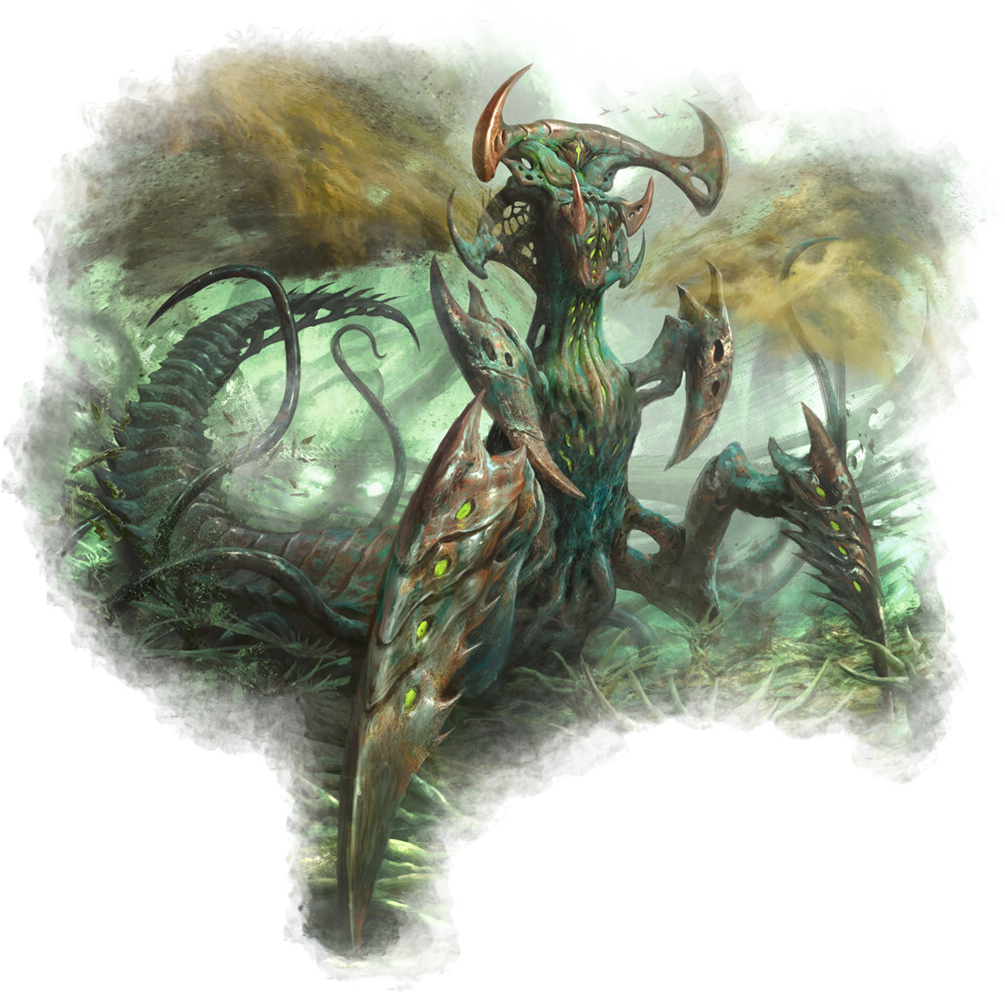
\includegraphics[width=1.3\columnwidth, height=280pt, keepaspectratio]{Scythera_Basilisk.png}%
      	\end{minipage}%
	};%
\end{tikzpicture}%
\addImageDBEntry{ToxicoreBasilisk3}{Page \thepage}{Art}{https://www.artofmtg.com/art/soprandrel-hunger-dominus/}{Soprandrel, Hunger Dominus MtG Art from Phyrexia: All Will Be One}{Antonio José Manzanedo}%

\begin{tikzpicture}[overlay, remember picture, inner sep=0pt, outer sep=0pt, path fading=fade down]%
	\node (posS) at (current page text area.south) {};%
	\node[below right=30pt and 4.4cm of posS, anchor=south] (cornerSE) {%
		\begin{minipage}{\columnwidth}%%
        	\centering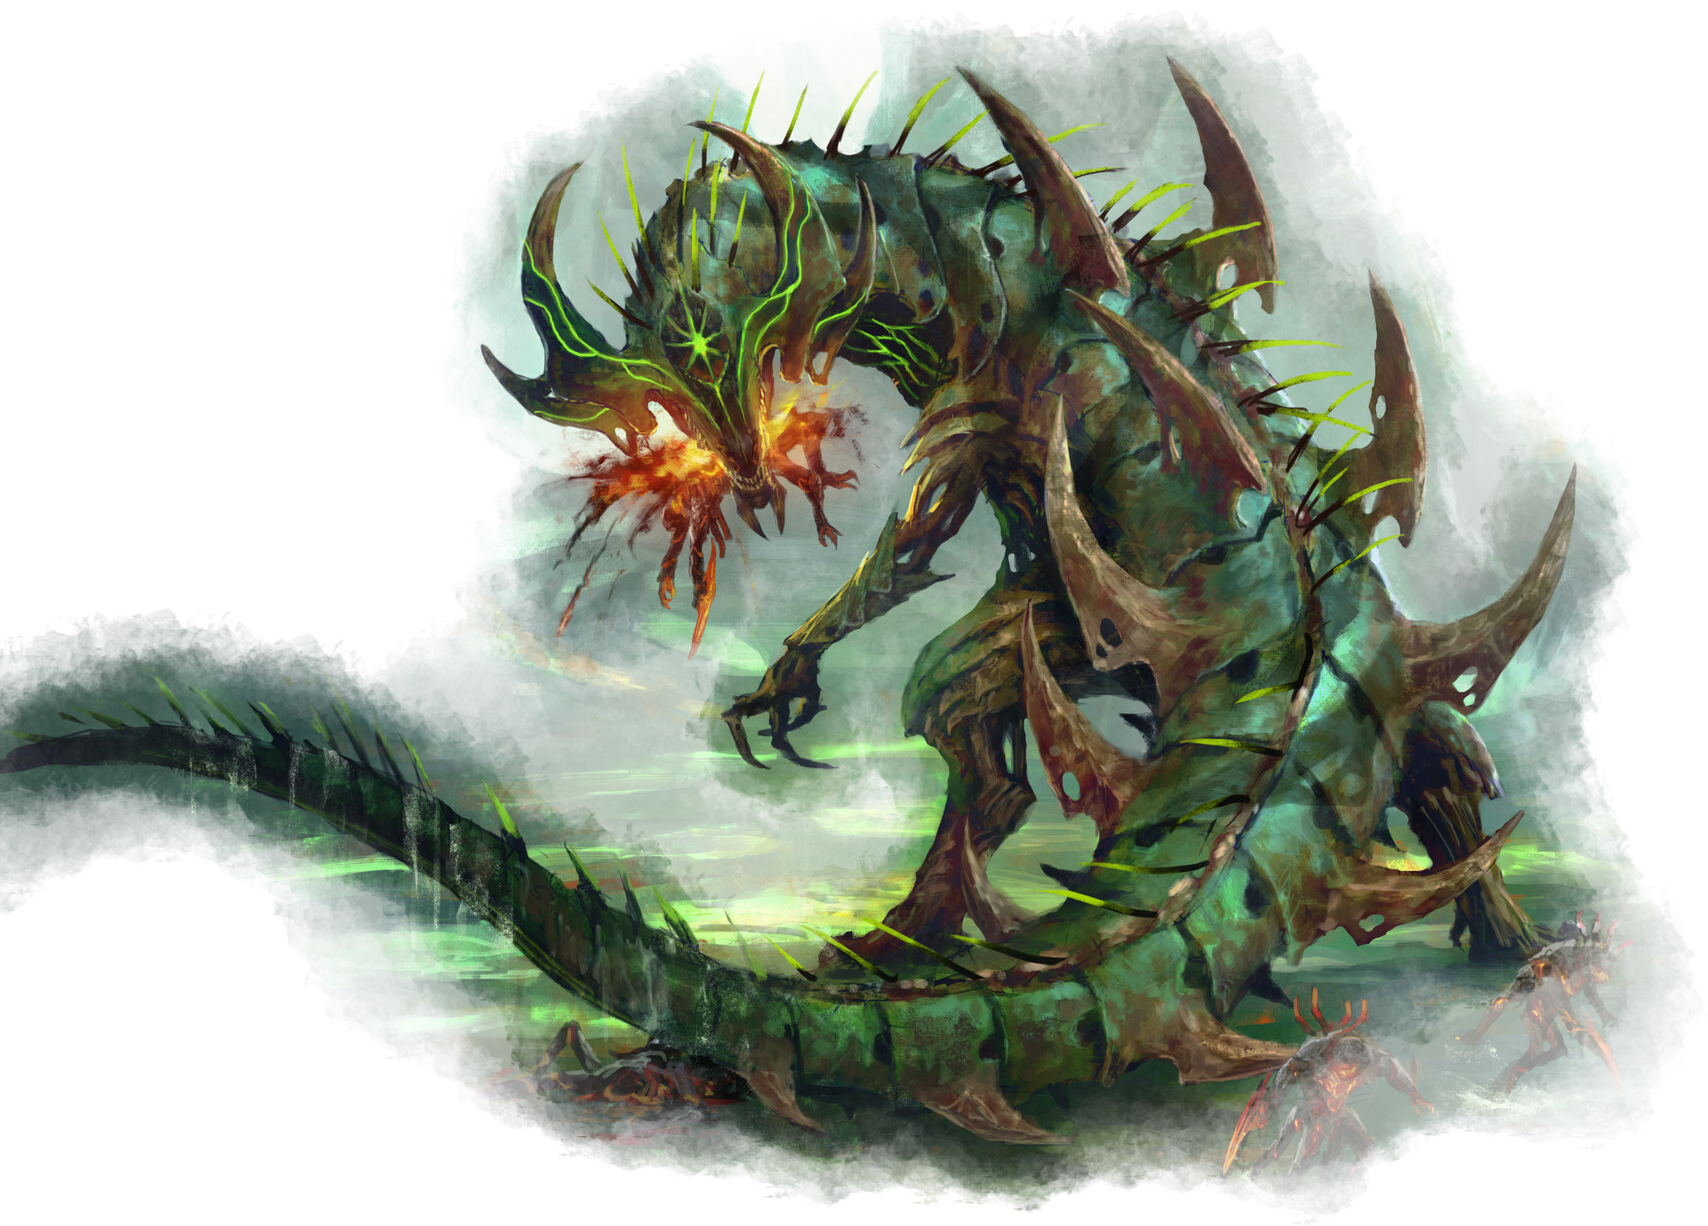
\includegraphics[width=1.3\columnwidth, height=250pt, keepaspectratio]{Bladescale_Basilisk.png}%
      	\end{minipage}%
	};%
\end{tikzpicture}%
\addImageDBEntry{ToxicoreBasilisk4}{Page \thepage}{Art}{https://www.artofmtg.com/art/tyrranax-rex/}{Tyrranax Rex MtG Art from Phyrexia: All Will Be One}{Tuan Duong Chu}%

% --------------------------------------------------------------------------------------------------- %
% ################################################################################################### %
% #-#-#-#-#-#-#-#-#-#-#-#-#-#-# Monster-Sheet with  full Footer-Graphic #-#-#-#-#-#-#-#-#-#-#-#-#-#-# %
% ################################################################################################### %
% --------------------------------------------------------------------------------------------------- %

\MonsterFooterGraphic{100pt}% offset for text to bottom
	{350pt}% max height of the image
	{Toxic_Forest(2).png}% image to be displayed as a banner
	{}% used for keepaspectratio for image ({} or {, keepaspectratio})
\addImageDBEntry{ToxicoreBasilisk5}{Page \thepage}{Background Art}{https://www.artofmtg.com/art/the-hunter-maze/}{The Hunter Maze MtG Art from Phyrexia: All Will Be One}{Alayna Danner}%

% Monster stat block
\vspace*{-1.3cm}\begin{DndMonster}[width=0.5\textwidth]{Vishgraz, the Toxicore Basilisk}
    \DndMonsterType{Huge Abomination, chaotic evil}

    % If you want to use commas in the key values, enclose the values in braces.
    \DndMonsterBasics[
        armor-class = {20 (natural armor)},
        hit-points  = {\DndDice{24d12 + 144}},
        speed       = {40 ft.},
    ]
    
    \renewcommand{\AbilityScoreSpacer}{~}

    \DndMonsterAbilityScores[
        str = 24,
        dex = 12,
        con = 22,
        int = 8,
        wis = 14,
        cha = 10,
    ]

    \DndMonsterDetails[
        saving-throws = {Dex +6, Con +11, Wis +8},
        skills = {Perception +12},
        %damage-vulnerabilities = {cold},
        damage-resistances = {Bludgeoning, Piercing, and Slashing from Nonmagical Attacks},
        damage-immunities = {Poison},
        condition-immunities = {Poisoned},
        senses = {Darkvision 120ft., Passive Perception 22},
        languages = {Common},
        challenge = 20,
    ]
    
    \DndMonsterAction{Legendary Resistance (3/Day)}
    If Vishgraz fails a saving throw, it can choose to succeed instead.
    
    \DndMonsterAction{Steelhide}
    The Scythera Basilisk has resistance to piercing, slashing, and bludgeoning damage from nonmagical attacks that aren't silvered.
    
    \DndMonsterAction{Keen Senses}
    The Scythera Basilisk has advantage on Wisdom (Perception) checks that rely on sight or smell.
    
    \DndMonsterAction{Toxic Aura}
    Any creature that starts its turn within 10 feet of Vishgraz must make a DC 20 Constitution saving throw, taking \DndDice{4d6} poison damage on a failed save, or half as much damage on a successful one.
	
	\DndMonsterSection{Actions}
	\DndMonsterAction{Multiattack}
	Vishgraz can make two Scythe Slash attacks and one Vicious Maw attack.
	
	\DndMonsterAttack[
      name=Scythe Slash,
      distance=melee, % valid options are in the set {both,melee,ranged},
      %type=weapon, %valid options are in the set {weapon,spell}
      mod=+14,
      reach=10,
      %range=20/60,
      targets=one target,
      dmg=\DndDice{3d8 + 7},
      dmg-type=slashing,
      plus-dmg=\DndDice{7d6},
      plus-dmg-type=poison,
      %or-dmg=,
      %or-dmg-when=,
      extra={. The target must succeed on a DC 20 Constitution saving throw or be poisoned for 1 minute. The poisoned creature can repeat the saving throw at the end of each of its turns, ending the effect on itself on a success},
    ]
    
    \DndMonsterAttack[
      name=Vicious Maw,
      distance=melee, % valid options are in the set {both,melee,ranged},
      %type=weapon, %valid options are in the set {weapon,spell}
      mod=+14,
      reach=10,
      %range=20/60,
      targets=one target,
      dmg=\DndDice{3d6 + 7},
      dmg-type=slashing,
      %plus-dmg=\DndDice{5d6},
      %plus-dmg-type=poison,
      or-dmg=\DndDice{6d6 + 7},
      or-dmg-when={if creature is already poisoned},
      %extra=,
    ]
    
    \DndMonsterAction{Corrosive Breath (Recharge 5-6)}
	Vishgraz exhales a 60-foot cone of corrosive gas. Each creature in that area must make a DC 20 Dexterity saving throw, taking \DndDice{12d6}) acid damage and \DndDice{12d6} poison damage on a failed save, or half as much damage on a successful one.
      
\end{DndMonster}

\vfill\eject % cammand to break to next column

%\nopagebreaksection{Blank Monster} % section that does not induce a new page
\hfil\\\vspace*{5cm}
\subsection*{Legendary Actions}
Vishgraz can take 3 legendary actions, choosing from the options below. Only one legendary action option can be used at a time, and only at the end of another creature's turn. Vishgraz regains spent legendary actions at the start of its turn.
\begin{DndMonsterLegendaryActions}
	\DndMonsterLegendaryAction{Toxic Spew}{Vishgraz targets a point it can see within 60 feet of it. The area becomes heavily obscured in a 20-foot radius until the end of Vishgraz's next turn. Each creature that starts its turn in that area takes \DndDice{3d6} poison damage.}
	\DndMonsterLegendaryAction{Terrifying Gaze}{Vishgraz fixes its gaze on a creature within 30 feet of it that can see it. If the target can see the basilisk's eyes, it must succeed on a DC 15 Wisdom saving throw or be frightened for 1 minute. The frightened creature can repeat the saving throw at the end of each of its turns, ending the effect on itself on a success. If a creature's saving throw is successful or the effect ends for it, the creature is immune to the Terrifying Gaze of all Toxicore Basilisks for the next 24 hours.}
	\DndMonsterLegendaryAction{Tail Sweep (Costs 2 Actions)}{Vishgraz sweeps its tail in a 20-foot cone. Each creature in that area must succeed on a DC 20 Dexterity saving throw or be knocked prone.}
\end{DndMonsterLegendaryActions}

\subsection*{Lair Actions}
On initiative count 20 (losing initiative ties), Vishgraz takes a lair action to cause one of the following effects:
\begin{itemize}
	\item The area becomes filled with a thick toxic mist, creating heavily obscured conditions. Each creature that is not a Toxicore Basilisk must make a DC18 Constitution Saving Throw or is poisoned for 1 minute.
	\item Poisonous vines erupt from the ground, creating difficult terrain. Each creature that is not a Toxicore Basilisk must make a DC16 Constitution Saving Throw or is poisoned for 1 minute.
	\item  The ambient temperature rises dramatically, causing all creatures in the area to make a DC 15 Constitution saving throw or take \DndDice{4d6} fire damage.
\end{itemize}

\begin{tikzpicture}[overlay, remember picture, inner sep=0pt, outer sep=0pt, path fading=fade down]%
	\node (posN) at (current page text area.north) {};%
	\node[above right=35pt and 10cm of posN, anchor=north east] (cornerNE) {%
		\begin{minipage}{\columnwidth}%%
        	\centering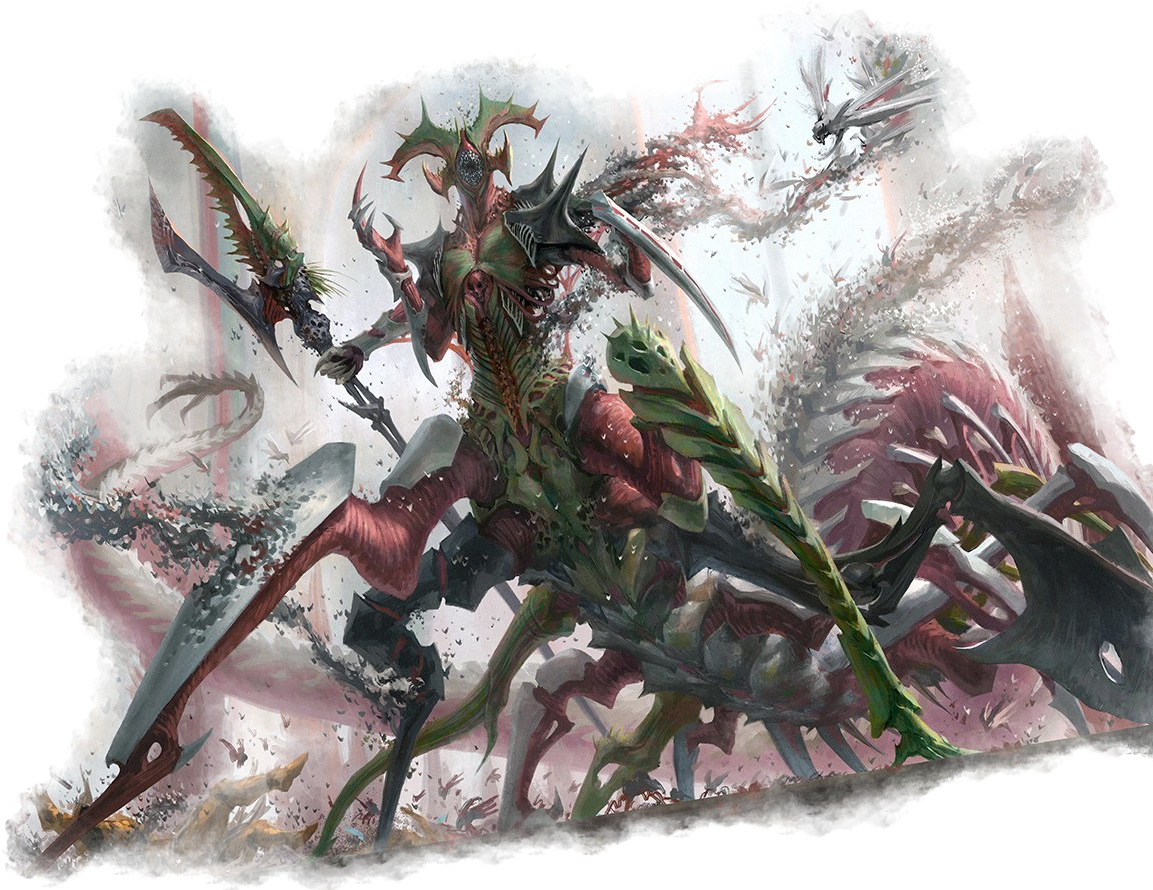
\includegraphics[width=1.1\columnwidth, height=280pt, keepaspectratio]{Vishgraz_Toxicore_Basilisk.png}%
      	\end{minipage}%
	};%
\end{tikzpicture}%
\addImageDBEntry{ToxicoreBasilisk6}{Page \thepage}{Monster Art}{https://scg-static.starcitygames.com/articles/2023/02/4da5b00e-vishgraz-the-doomhive-700x547.jpg}{Vishgraz, the Doomhive MtG Art from Phyrexia: All Will Be One}{Andrew Mar}%

\end{document}
